% !TeX program = xelatex
\documentclass{article}
\usepackage{xeCJK}
\usepackage{tikz}
\usepackage[outline]{contour}
\usepackage{graphicx}
\graphicspath{ {./} }
\setCJKmainfont{Kaiti SC}
% \setCJKmainfont{Xingkai SC}
% \setCJKmainfont{STKaiti}

\newcommand\Grid[1]{%
 \tikz[baseline=(char.base)]{%
  \draw[xstep=1ex,ystep=1ex,help lines] (-1ex,-1ex) grid (1ex,1ex);
  \draw[help lines,densely dash dot]
  (-1ex,-1ex) -- (1ex,1ex)  (-1ex,1ex) -- (1ex,-1ex);
  \node[inner sep=0pt] (char) at (0,0) {#1};
 }%
}
\pagenumbering{gobble}
\begin{document}
\begin{center}
    \Huge 咏柳 \\
\end{center}
\begin{flushright}
    \huge 唐 $\bullet$ 贺知章 \\
\end{flushright}
\begin{center}
    \Huge 碧玉妆成一树高 \\
    \Huge 万条垂下绿丝绦 \\
    \Huge 不知细叶谁裁出 \\
    \Huge 二月春风似剪刀 \\
\end{center}
\hrule
\begin{center}
    \Huge \Grid{咏}\Grid{柳} \\
\end{center}
\begin{flushright}
    \huge \Grid{唐} $\bullet$ \Grid{贺}\Grid{知}\Grid{章} \\
\end{flushright}
\begin{center}
    \Huge \Grid{碧}\Grid{玉}\Grid{妆}\Grid{成}\Grid{一}\Grid{树}\Grid{高} \\
    \Huge \Grid{万}\Grid{条}\Grid{垂}\Grid{下}\Grid{绿}\Grid{丝}\Grid{绦} \\
    \Huge \Grid{不}\Grid{知}\Grid{细}\Grid{叶}\Grid{谁}\Grid{裁}\Grid{出} \\
    \Huge \Grid{二}\Grid{月}\Grid{春}\Grid{风}\Grid{似}\Grid{剪}\Grid{刀} \\
\end{center}
\hrule
\newpage
\begin{figure}
    \centering
    \makebox[0pt]{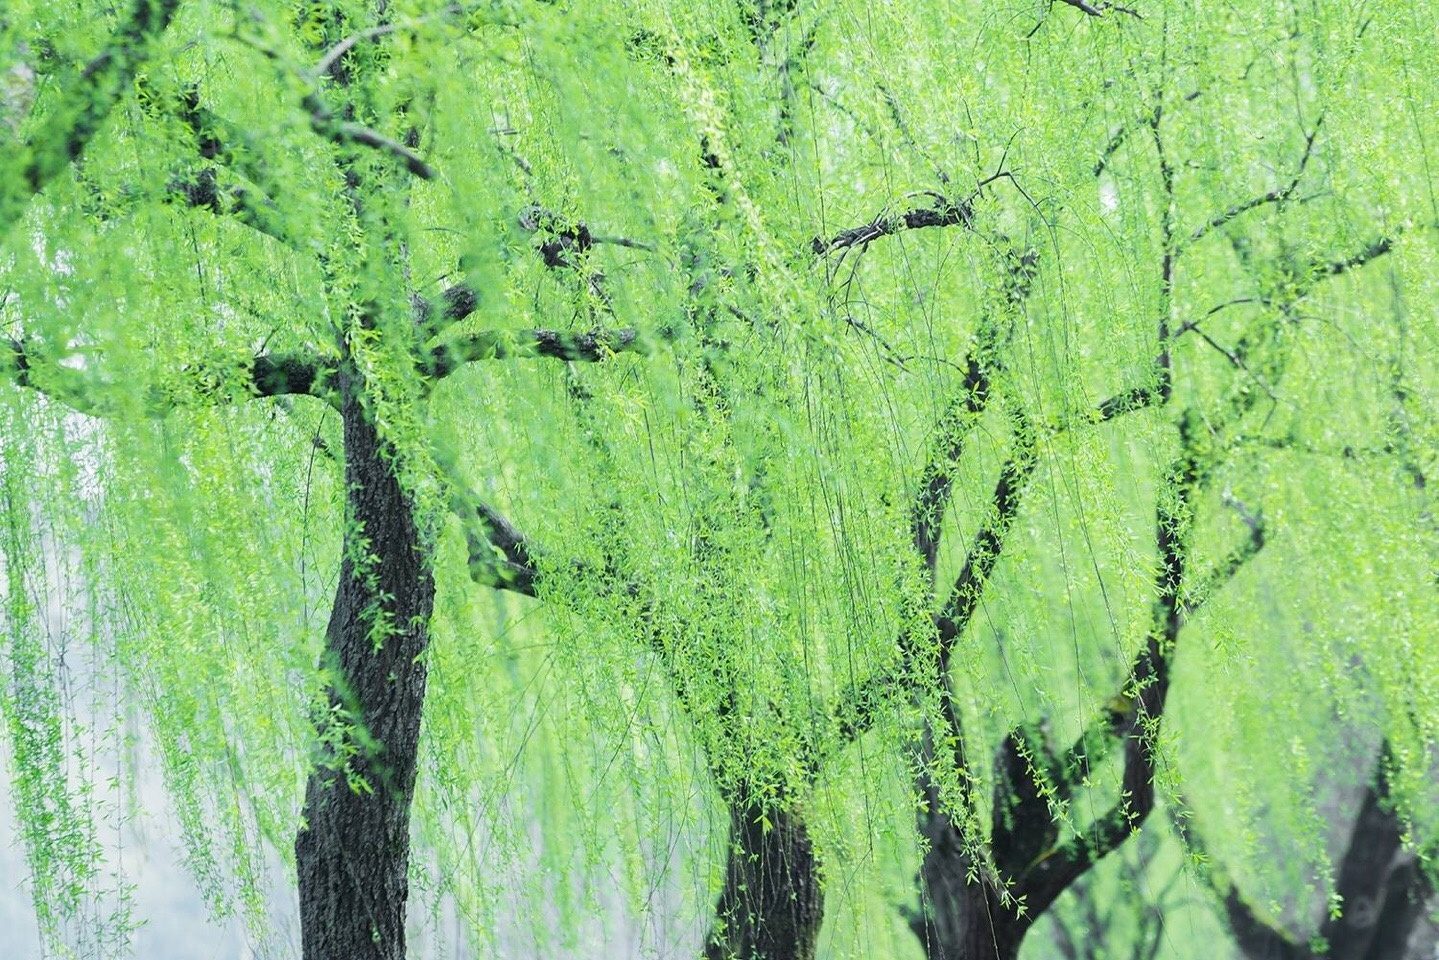
\includegraphics[width=0.9\paperwidth]{image1.jpeg}}
\end{figure}
\begin{figure}
    \centering
    \makebox[0pt]{
\includegraphics[width=0.9\paperwidth]{image2.jpeg}}
\end{figure}
\end{document}
